%!TEX root = main.tex

We evaluate the performances of our structured attention model
and structured entailment model on the Stanford
Natural Language Inference (SNLI) dataset \cite{bowman2015large}.
The SNLI dataset
contains $\sim570$k sentence pairs.
%Each pair is labeled with one of the relations of
%entailment, neutral, contradiction and $-$,
%where $-$ means there is no consensus among the annotators.
%All those sentence pairs with $-$ labels are discarded.
We use the binarized trees in SNLI dataset in our experiments.

\begin{figure*}[ht]
\begin{center}
\begin{tabular}{cc}
\raisebox{0pt}{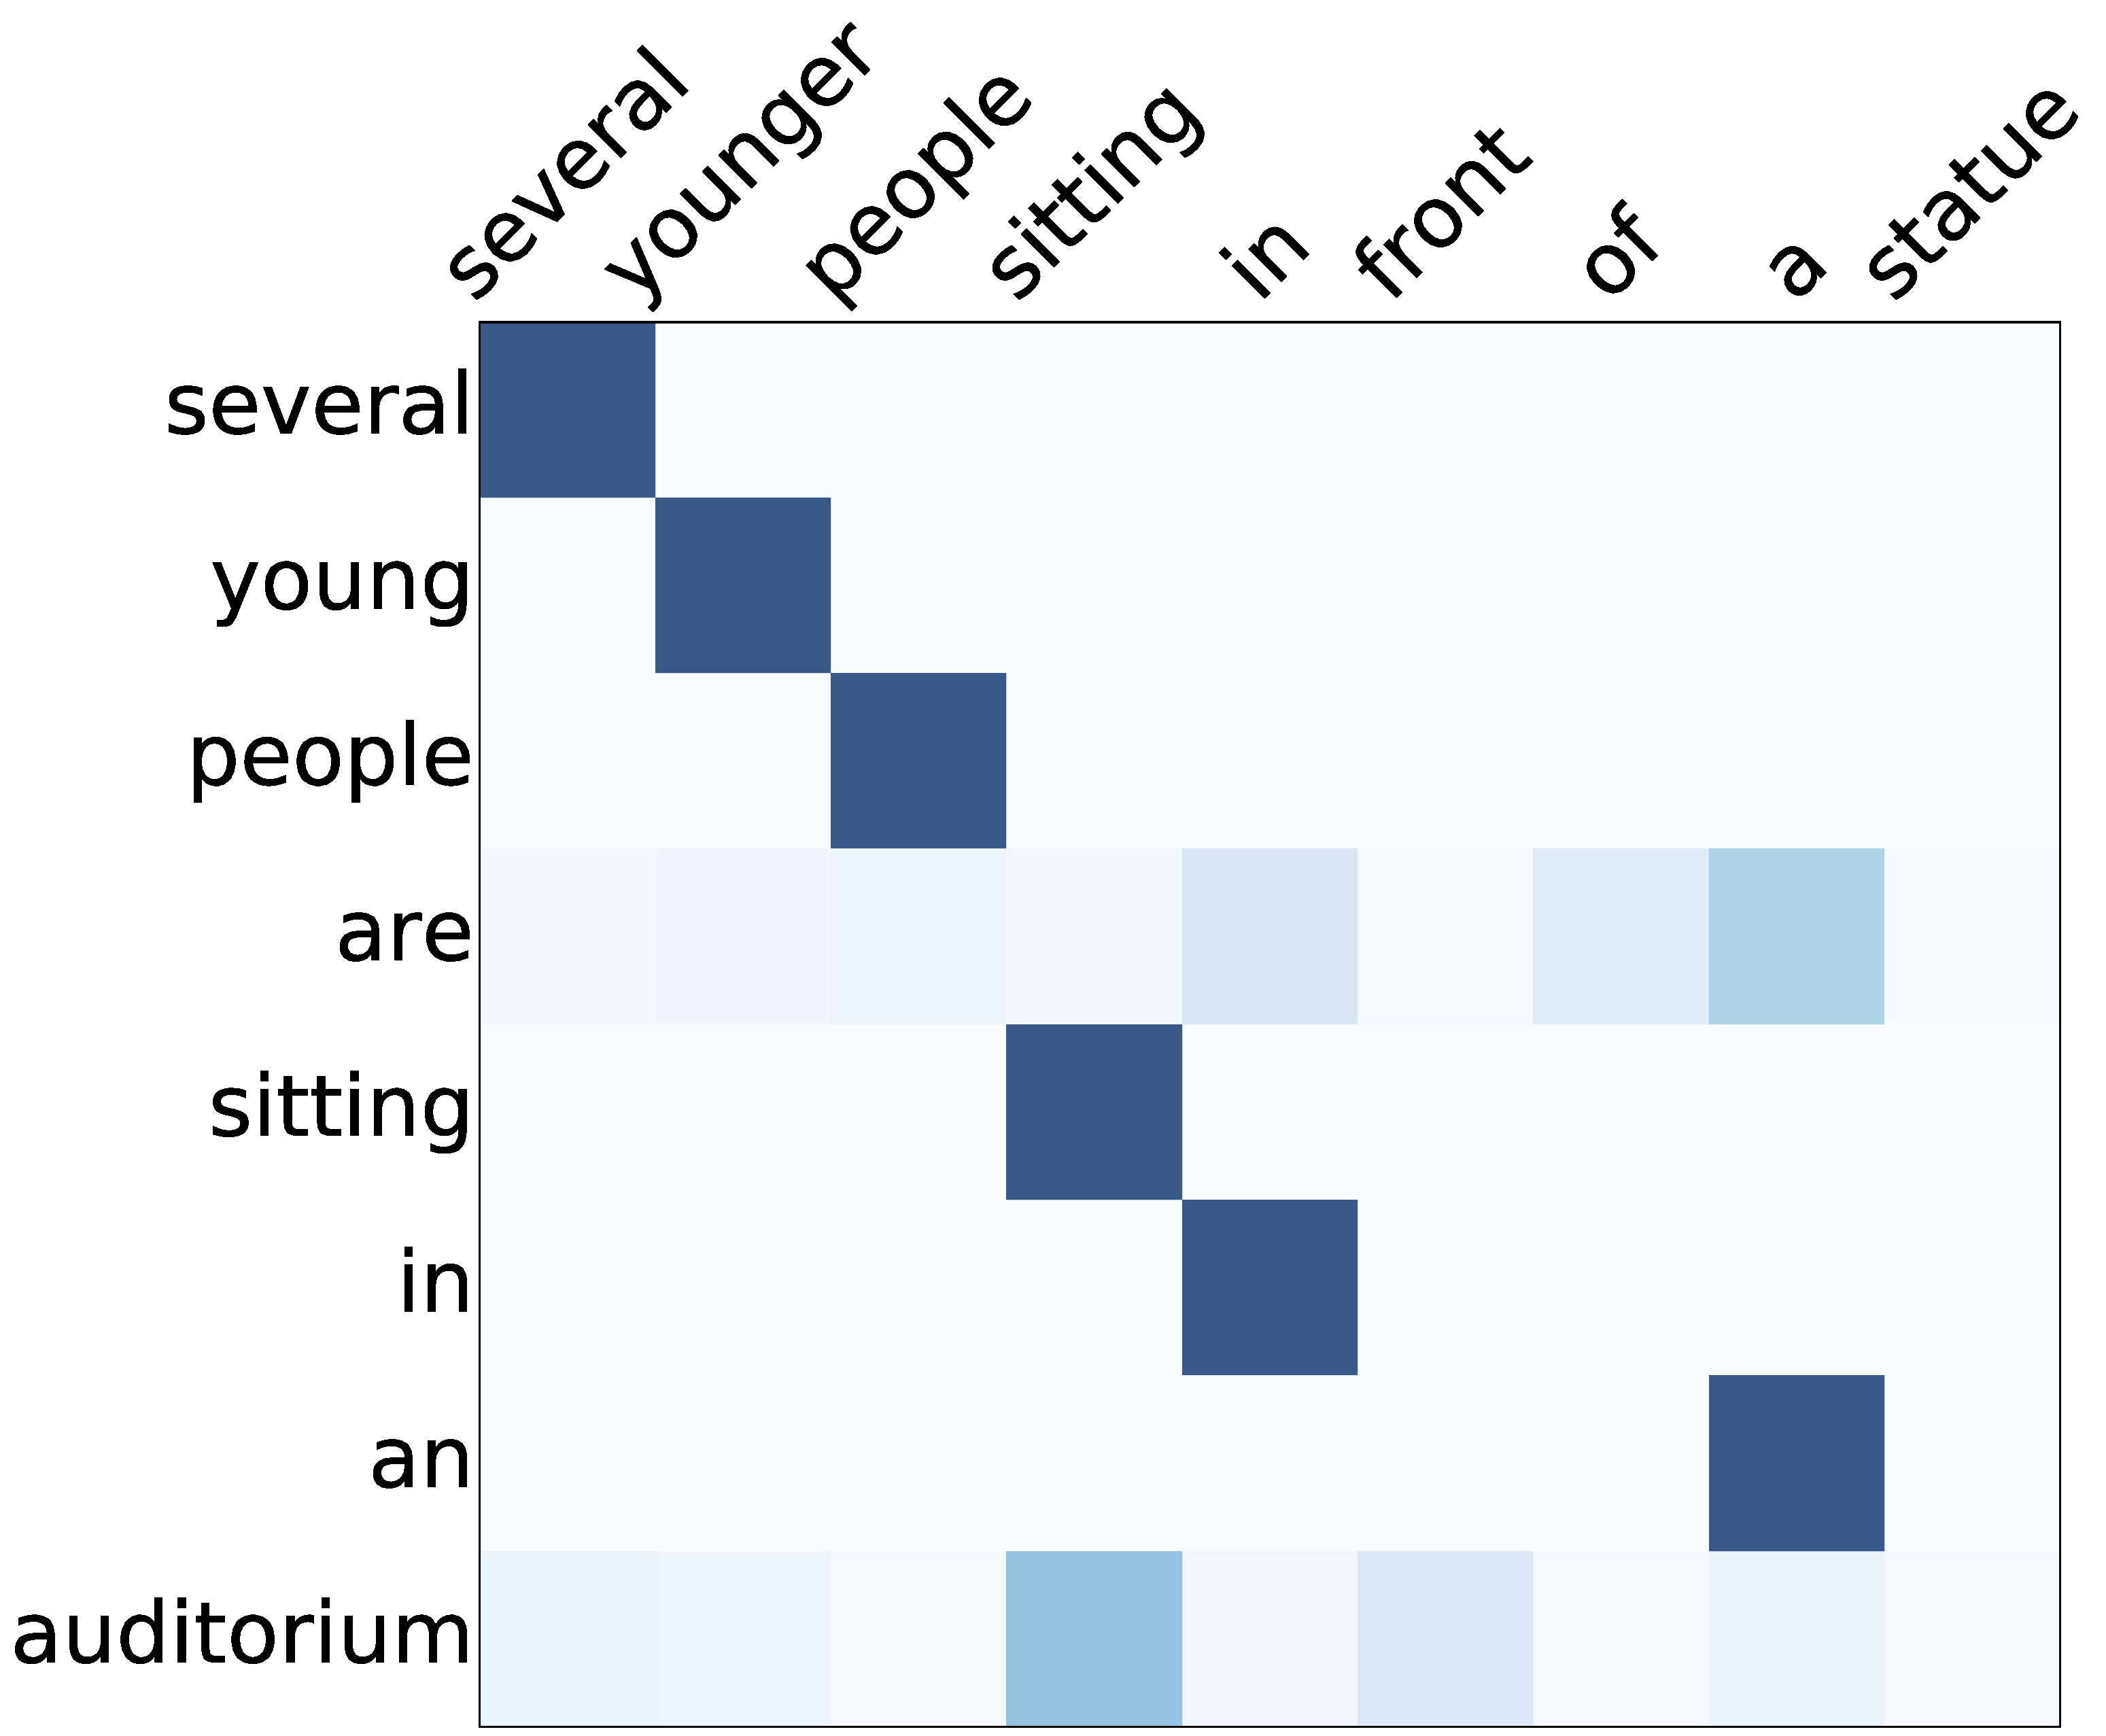
\includegraphics[width=0.35\textwidth]{test.232.align.pdf}} &
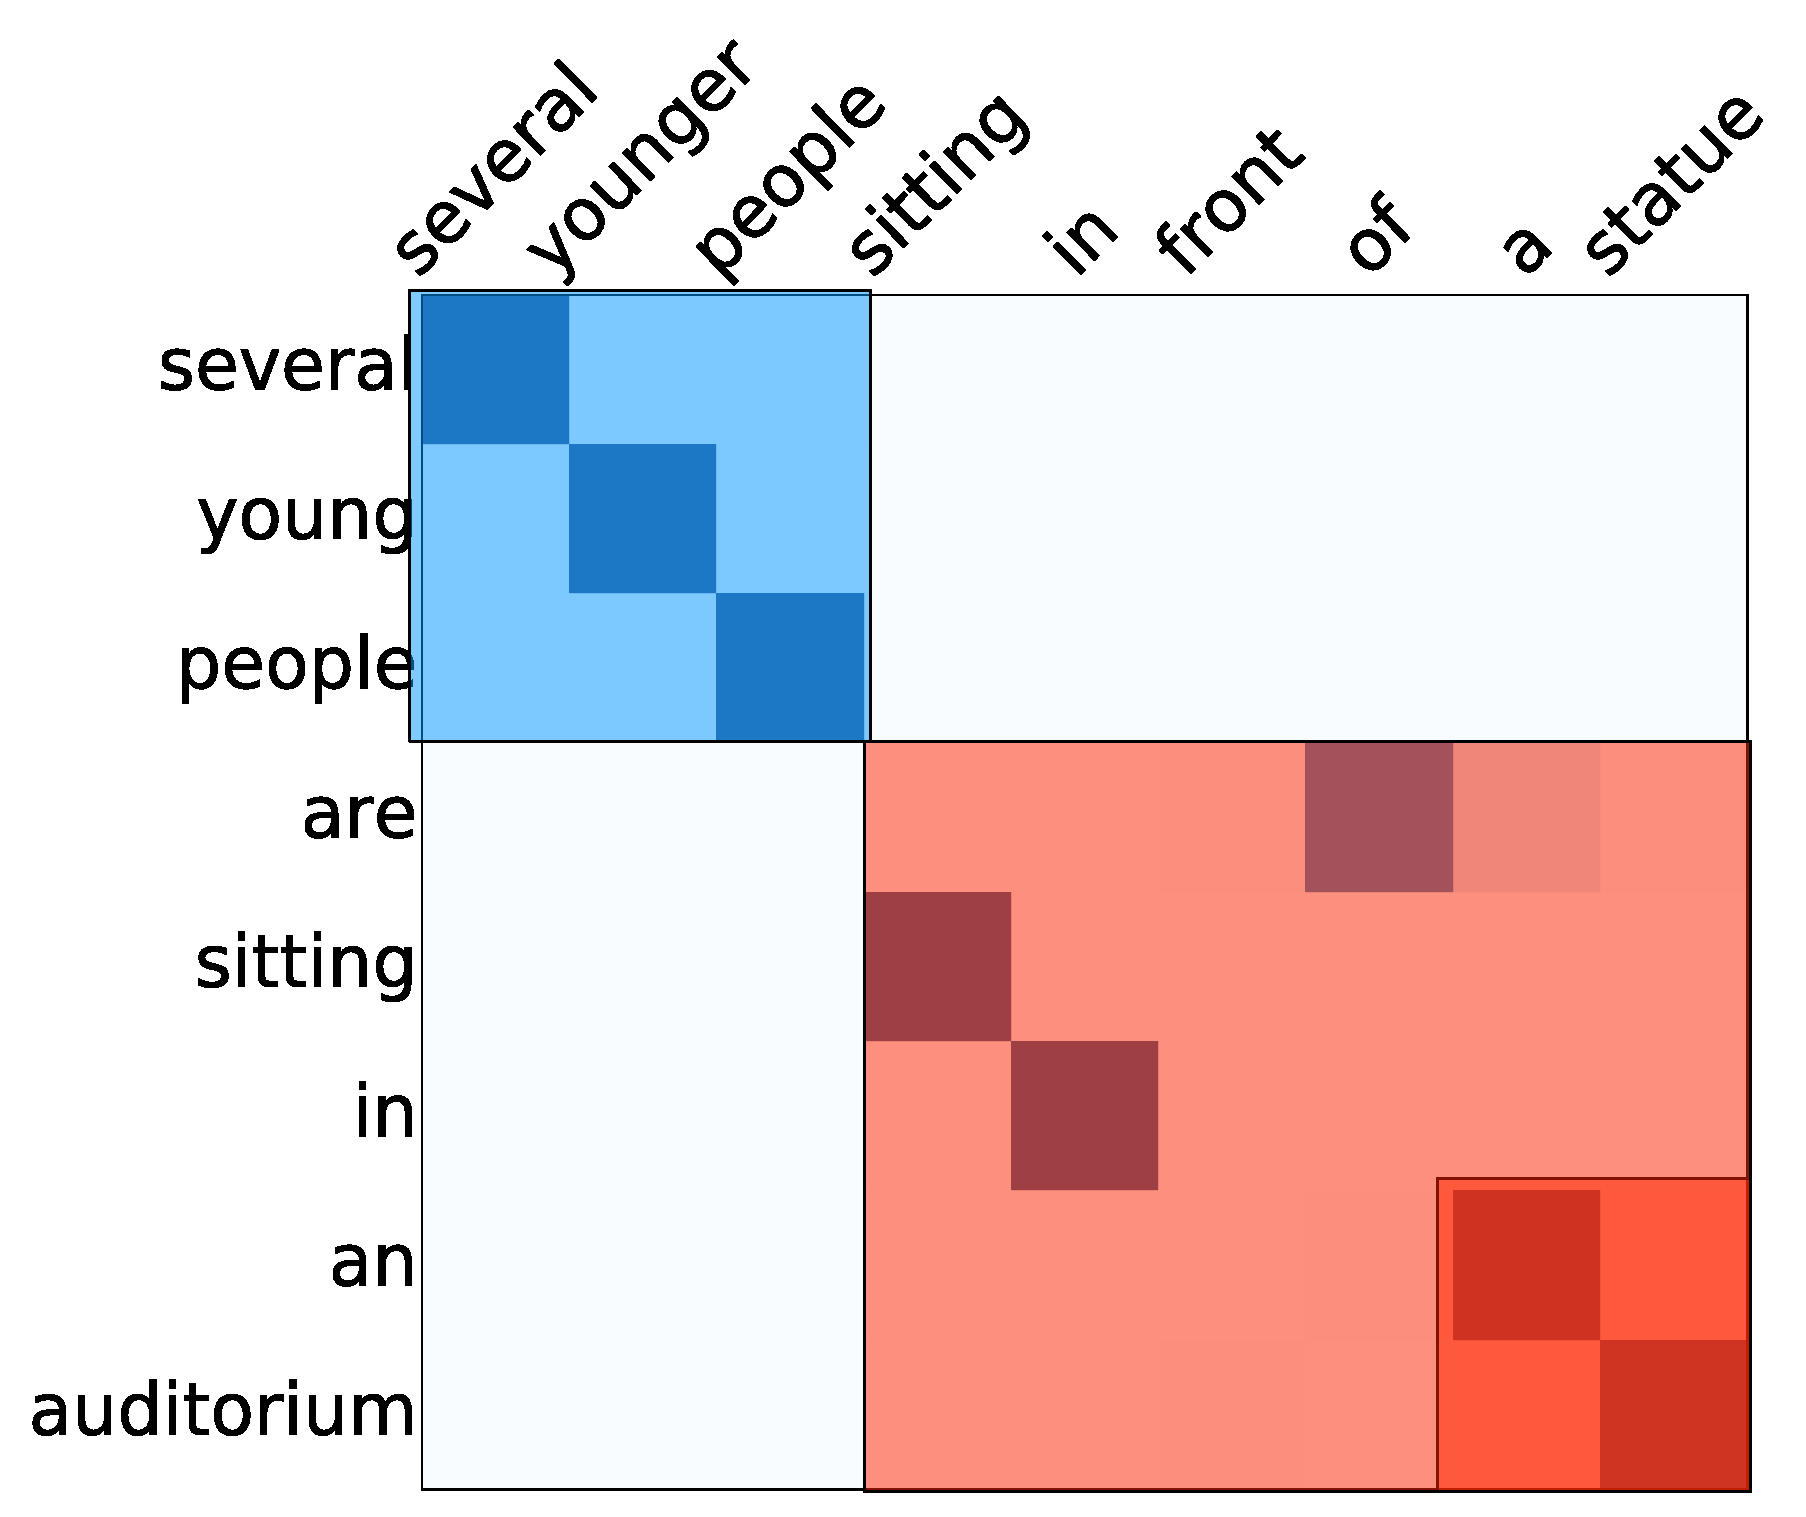
\includegraphics[width=0.35\textwidth]{test.232.dual.align} \\
(a) attention & (b) dual-attention\\
\raisebox{0pt}{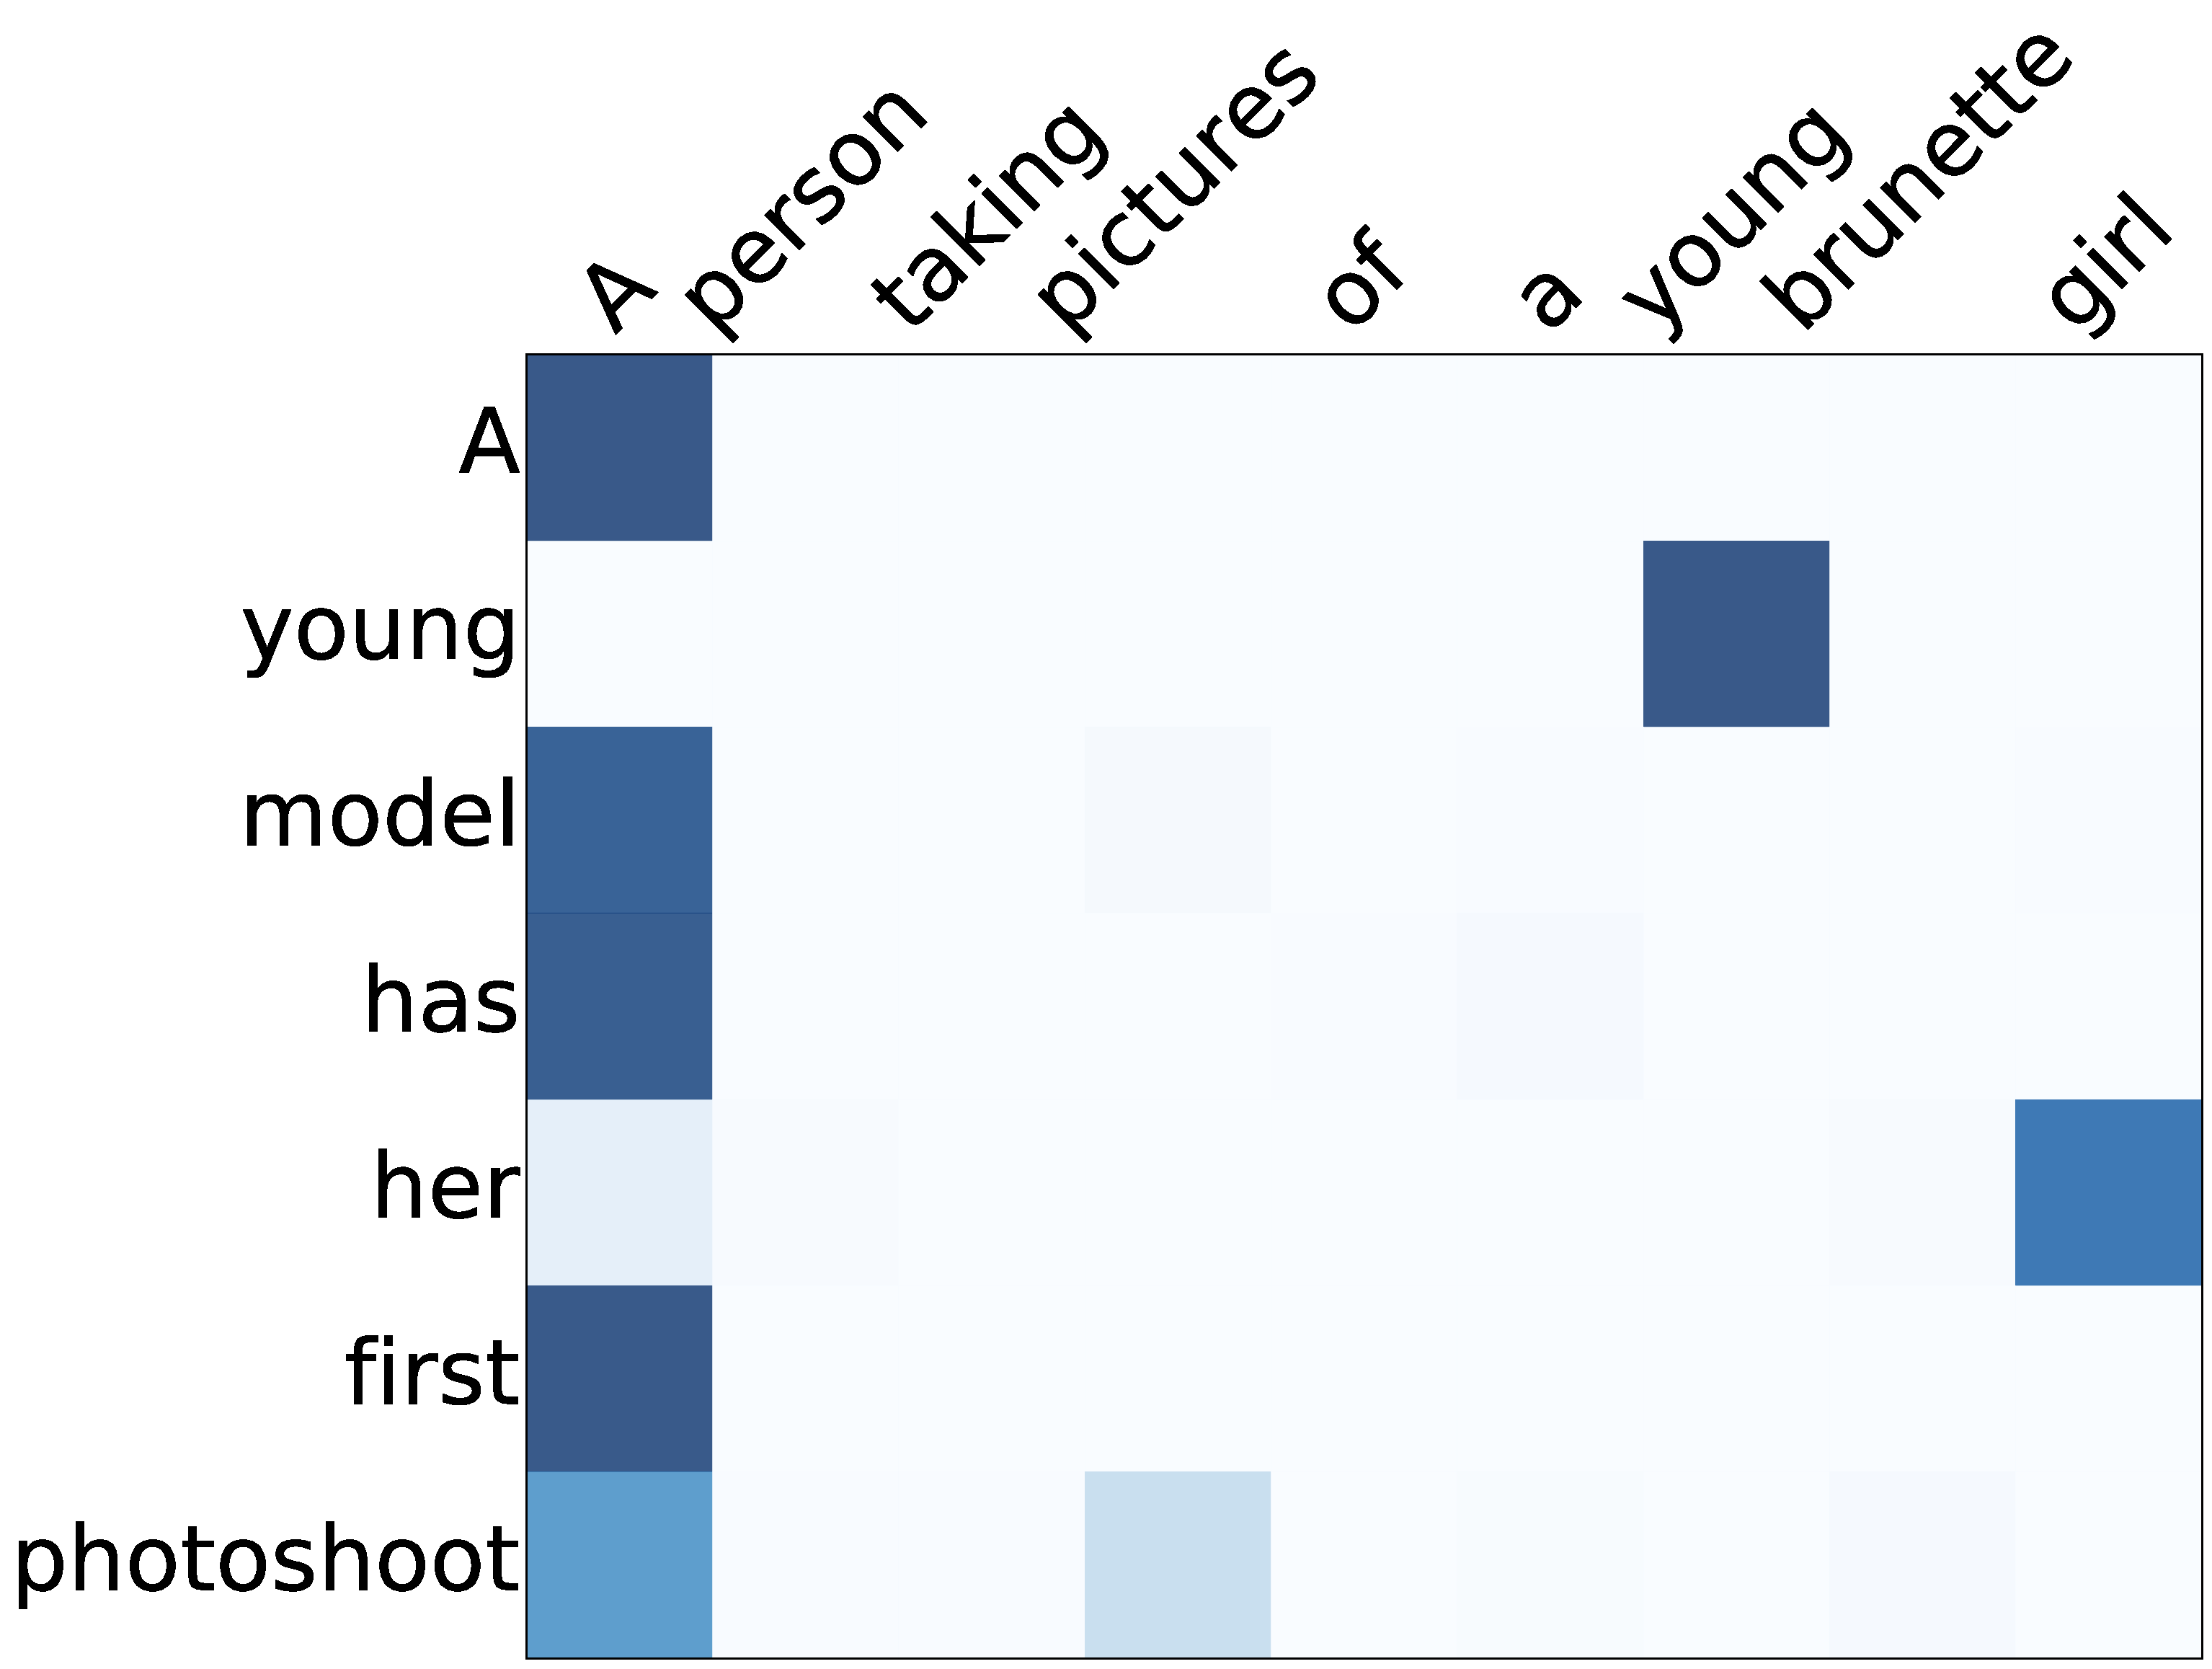
\includegraphics[width=0.35\textwidth]{test.1598.align.pdf}} &
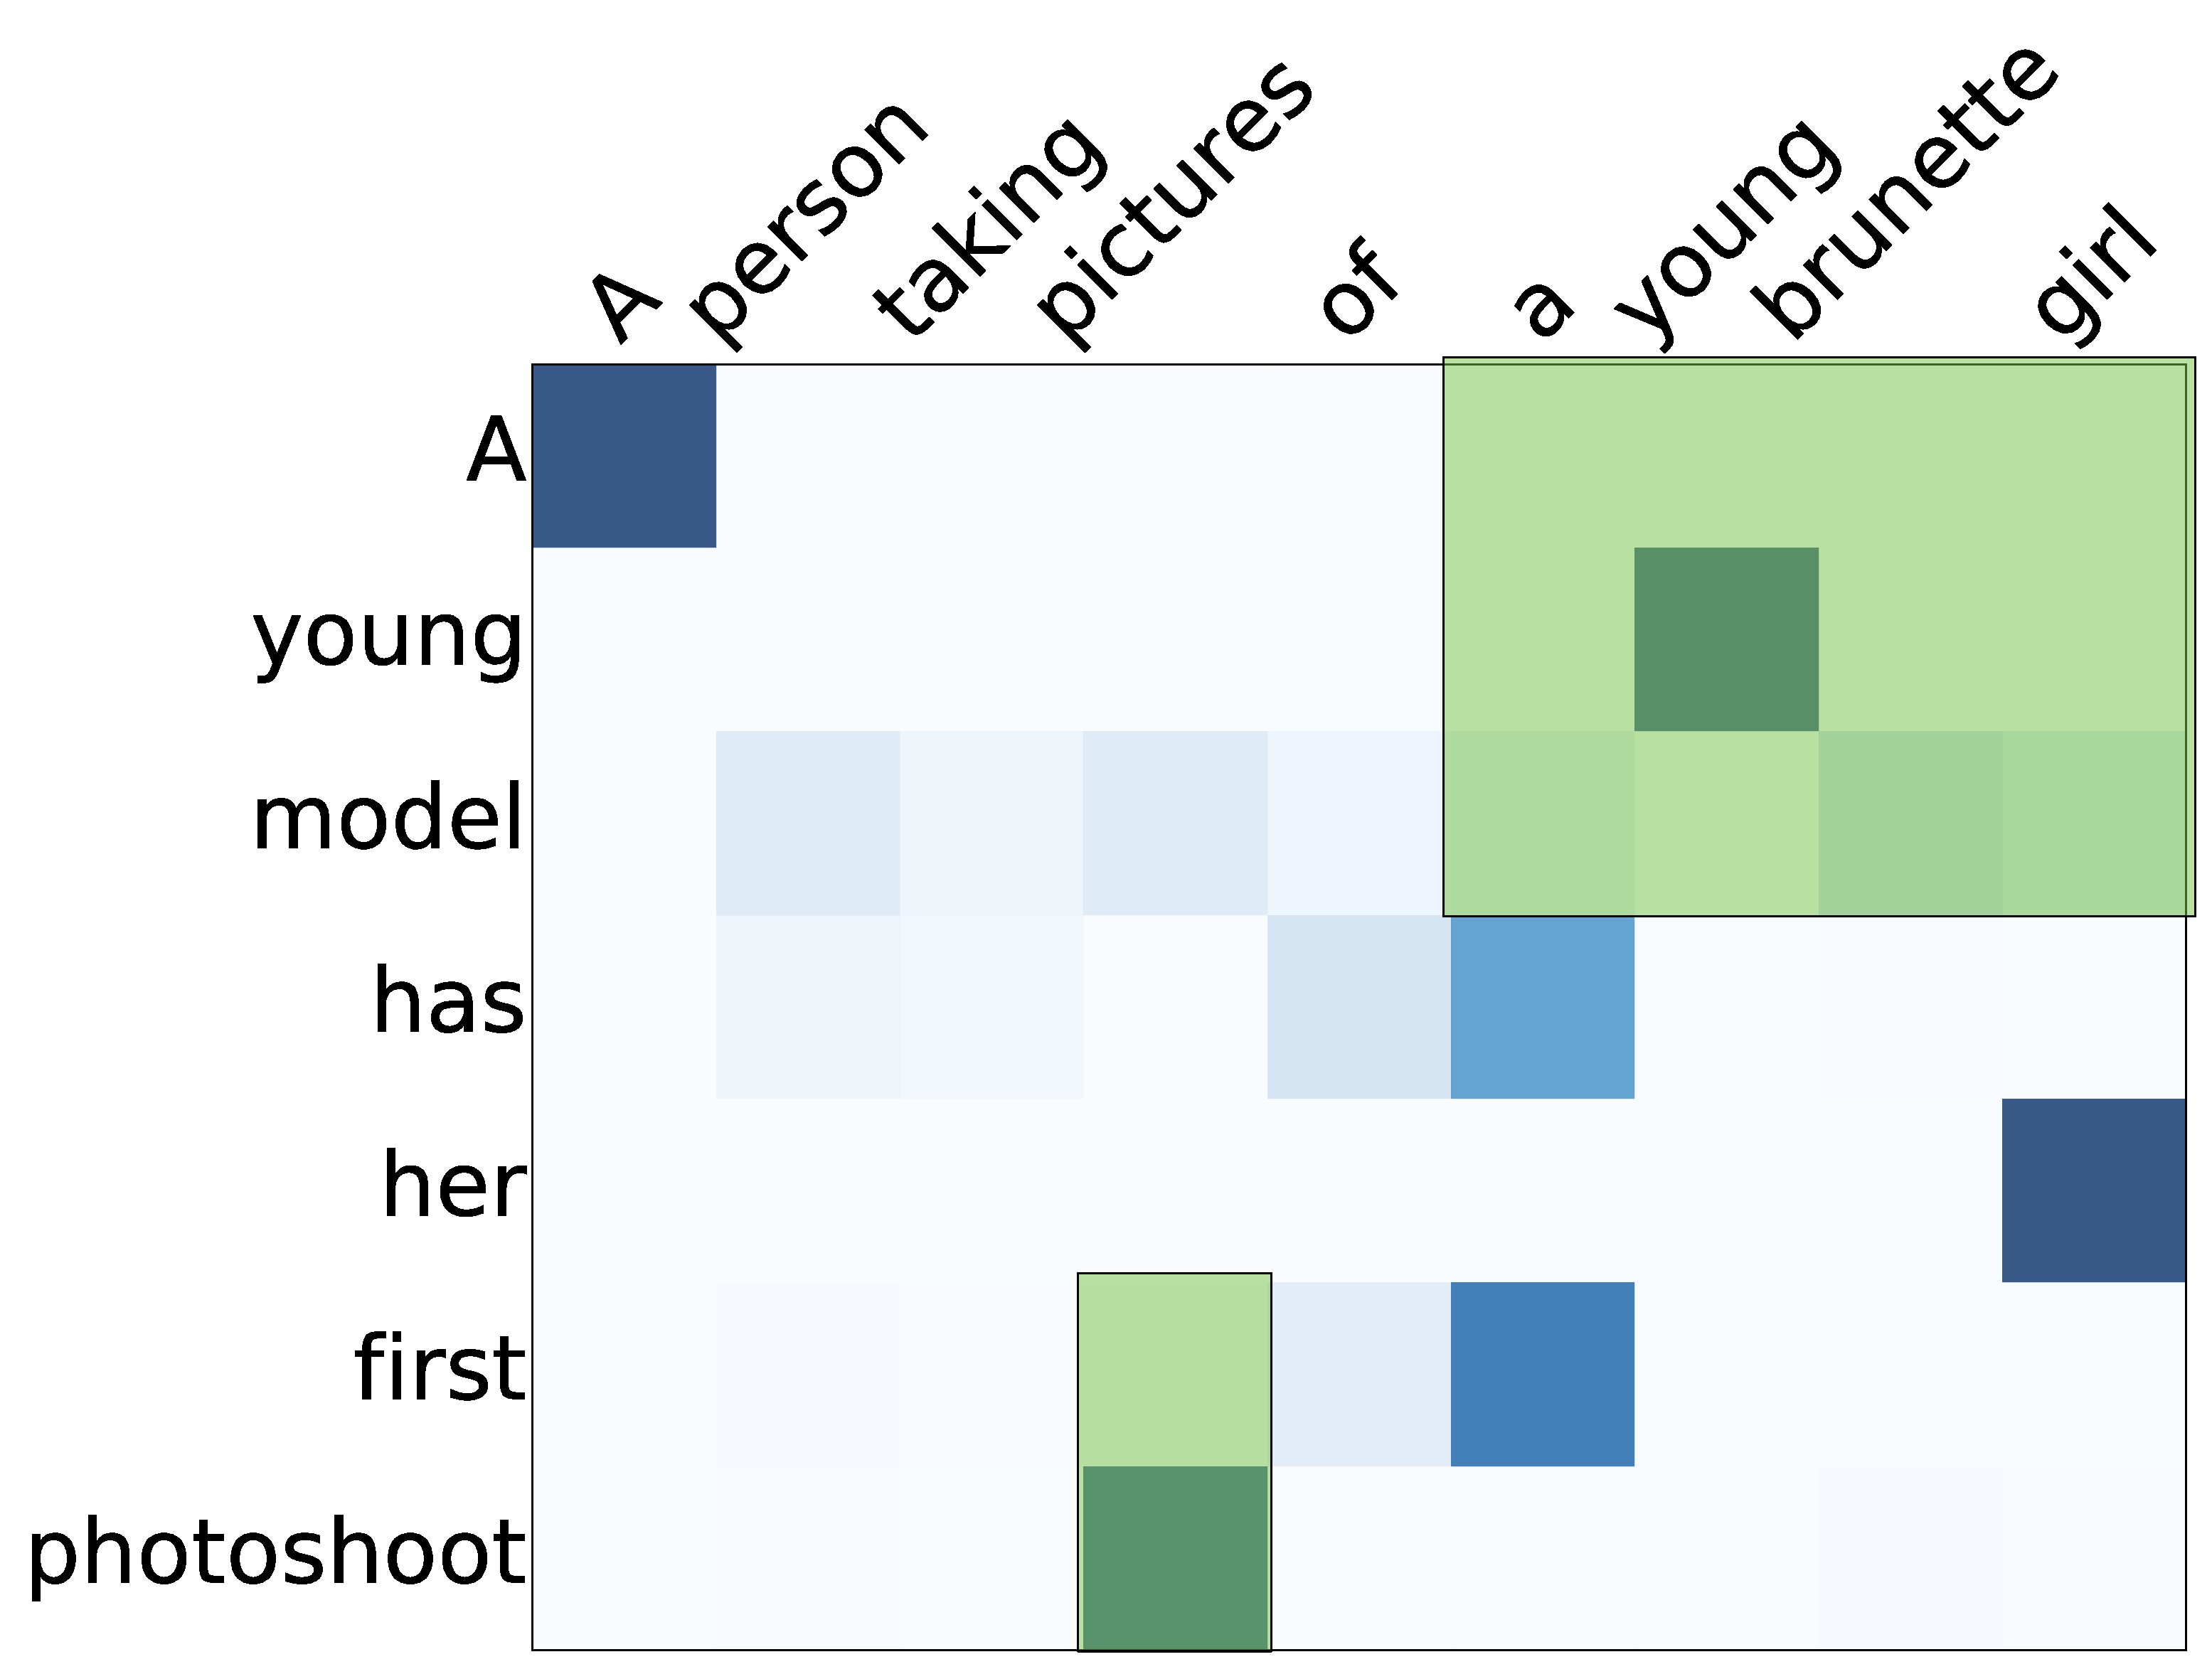
\includegraphics[width=0.35\textwidth]{test.1598.dual.align} \\
(c) attention & (d) dual-attention\\
\end{tabular}
\end{center}
%\vspace{-0.2cm}
\caption{Attention matrices for exemplary sentence pairs.
Note that, for brevity we {\it only show} the attentions 
between each word pair, and skip
the attentions of tree nodes.
Some important tree node alignments calculated by our model are highlighted 
using the colored boxes,
where the colors of the boxes represent the entailment relations (see
Figure~\ref{fig:ent-example}).
(a) (b) Premise: several younger people sitting in front of a statue. Hypothesis: several young people sitting in an auditorium.
Dual-attention fixes the misaligned word ``auditorium''.
(c) (d) Premise: A person taking pictures of a young brunette girl.
Hypothesis: A young model has her first photoshoot. 
Dual-attention fixes the uncertain alignments for ``photoshoot''
and ``model''.
\label{fig:align-example}}
%\vspace{-0.5cm}
\end{figure*}

\begin{figure*}[ht]
\begin{center}
\begin{tabular}{c}
%\vspace{-0.2cm}
\raisebox{1.5in}{(a)}
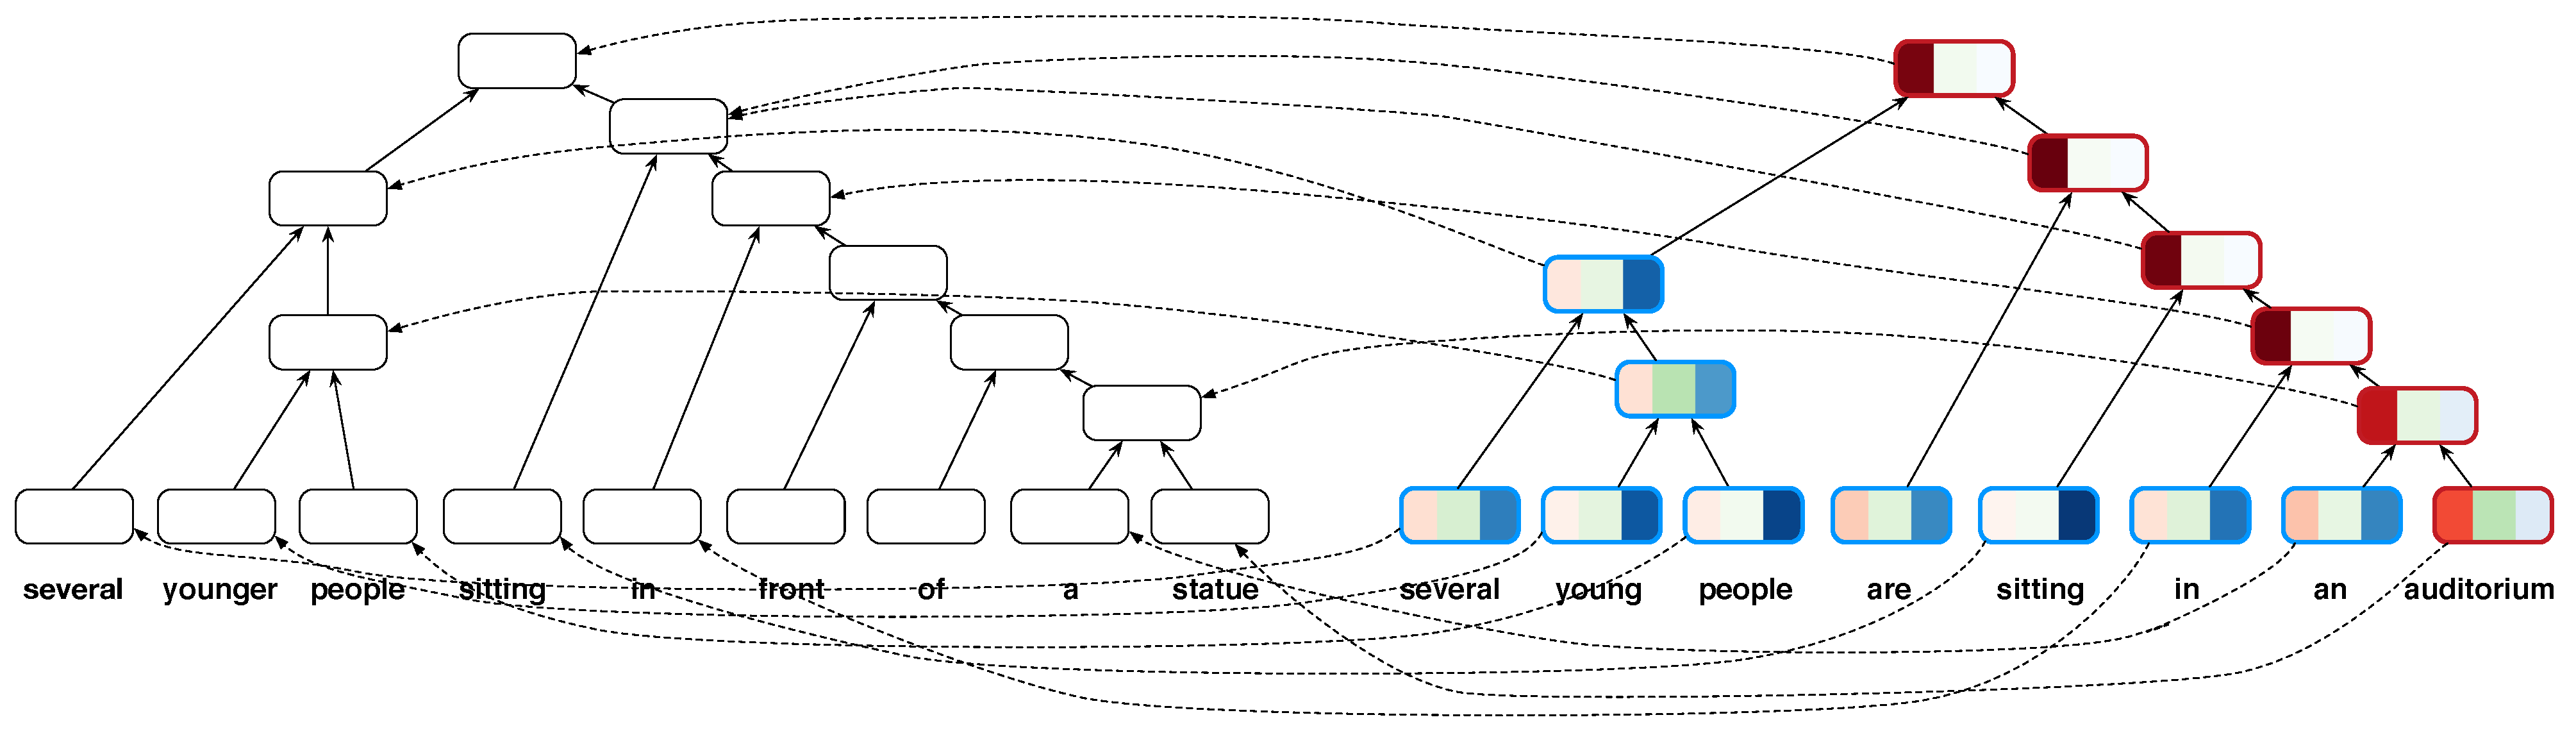
\includegraphics[width=0.97\textwidth]{test.232.ent}\\
%\vspace{-0.1cm}
%(a) \\
\raisebox{1.5in}{(b)}
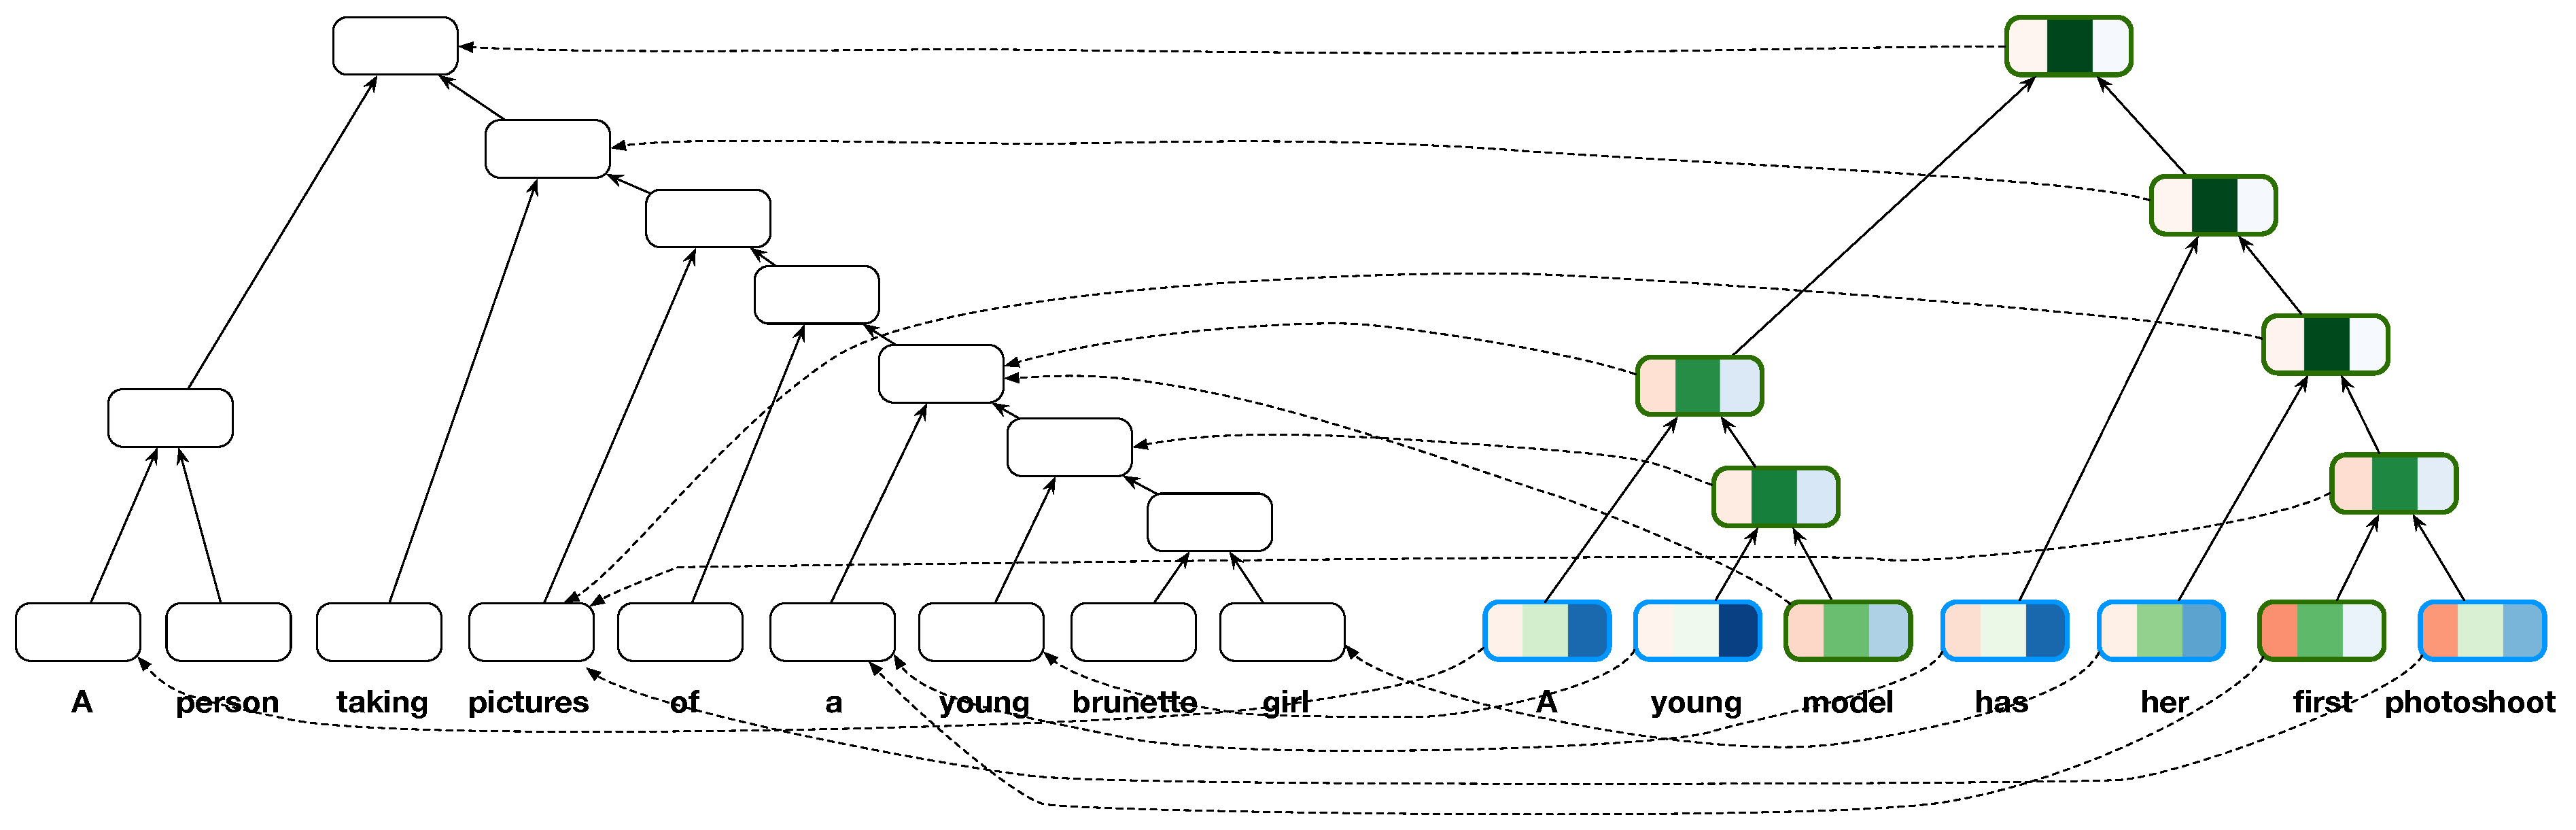
\includegraphics[width=0.97\textwidth]{test.1598.ent}% \\
%\vspace{-0.2cm}
%(b)
\end{tabular}
\end{center}
%\vspace{-0.5cm}
\caption{Examples illustrating entailment relation composition.
(a) for Figure~\ref{fig:align-example} (b); (b) for Figure~\ref{fig:align-example} (d). 
For each hypothesis tree node, the dashed line shows
to its most confident alignment.
The three color stripes in each node indicate
the confidences of the corresponding entailment relation
estimation: red for {\color{red} contradiction}, 
green for {\color{green} neutral}, and blue for {\color{blue} entailment}.
The colors of the node borders show the dominant 
estimation.
Note: there is no strong alignment for hypothesis word ``are'' in (a).
\label{fig:ent-example}}
%\vspace{-0.4cm}
\end{figure*}

%\vspace{-0.3cm}
\subsection{Experiment Settings}


{\bf Network Architecture}

The general structure of our model is illustrated 
in Figure~\ref{fig:arch}.
We omitted a dropout layer between the word embedding 
layers and the tree LSTM layers in Figure~\ref{fig:arch}.
%at the bottom there is a embedding layer that maps 
%each natural language sentence to a sequence
%of word embedding vectors. 
%The output of this layer is then passed to a dropout layer.
%After the dropout
%the result is fed into a Binary-Tree LSTM to generate
%meaning representations for each tree node.
%The Alignment Module (Section~\ref{sec:att})
%calculates the expected alignment (attention)
%based on the node meaning representation.
%The Entailment Composition Module (Section~\ref{sec:ent})
%uses the expected alignment and the tree node meaning representations
%to compute the entailment relation representation
%along the hypothesis tree from bottom up,
%and the final result is passed to a softmax layer
%to calculate the probabilities for each of the 3 relations.
We use cross-entropy as the training objective.\footnote{
Our code is released at \url{https://github.com/kaayy/structured-attention}.}

%We implement our system using {\tt torch}.


\noindent {\bf Parameter Initialization \& Hyper-parameters}

We use GloVe \cite{pennington2014glove} to initialize the 
word embedding layer. In the training we do not change the embeddings,
except for the OOV words in the training set.
For the parameters of the rest layers,
we use a uniform distribution between $-0.05$ and $0.05$
as initialization.

Our model is trained in an end-to-end manner with adam \cite{kingma2014adam} as the optimizer.
We set the learning rate to 0.001, $\beta_1$ to 0.9,
and $\beta_2$ to 0.999.
We use minibatch of size 32 in the training.
The dropout rate is 0.2.
The length for the Tree-LSTM meaning representation
$k=150$. The length of the entailment relation
vector $r=150$.

%\vspace{-0.3cm}
\subsection{Quantitative Evaluation}




We present a comparison of structured model with existing methods
of LSTM-based sentence embedding \cite{bowman2015large},
LSTM with attention \cite{rocktaschel2015reasoning},
Binary Tree-LSTM sentence embedding (our implementation
of \newcite{tai2015improved}),
mLSTM \cite{wang2015learning},
and LSTM-network \cite{cheng2016long} 
in Table~\ref{tab:results}.

%We start with introducing Binary-Tree LSTM for sentence 
%meaning representation to \cite{bowman2015large}. 
%This meaning representation
%is then feed directly into an NN similar to \cite{bowman2015large}.
%With this simple replacement of the sentence meaning representation
%brings $\sim$1.5 improvement to 79.9 in the test set,
%which reveals the potential of learning sentence representations
%with sentence structures.

We first try Binary-Tree LSTM with a composition function
$f_{\text{rel}}$ of a 
recurrent network with attention as 
in \newcite{rocktaschel2015reasoning},
which achieves an accuracy of 81.8.
%based on the Binary-TreeLSTM sentence embedding.
%By checking the training statistics 
%(e.g., the norm of the gradient passed between the
%network layers), we find that
%this network has the vanishing gradient issue,
%which might explain why it does not perform as well
%as the same RNN in the sequence model.
We find the training of this RNN is difficult due
to the vanishing gradient problem.

Using Binary-Tree LSTM for entailment relation composition
instead of the simple RNN brings $\sim$4.6 improvement. 
%We observe that the gradients passed between the network
%layers are usually 2 orders of magnitude larger 
%than the simple RNN model, which might explain
%the superior performance.
We observe that the vanishing gradient problem is greatly
alleviated.
Dual-attention further improves the tree
node alignment, achieving another 0.8 improvement.

%Comparing with other LSTM-based methods, %in the same task,
Our structured entailment composition model outperforms
the similar mLSTM model, which essentially
also uses an LSTM layer to propagate 
the ``matching'' information, but sequentially. %not
%in the bottom-up order.
With the help of dual-attention, our model outperforms
mLSTM with a 1.1 point margin.

%LSTM-network model \cite{cheng2016long}
%applies attention within the 
%sentence, 
%which is orthogonal to our work. 
%Ideally we can also integrate the intra-sentence
%attention to our model. We leave this as further work.
 

%%%%%%%%%%%%%%%%%%%%%%%%%%%%%%%%%%%%%%%%%%%
%\vspace{-0.3cm}
\subsection{Qualitative Evaluation}
\label{sec:qual-eval}


Due to space constraints, 
here we highlight two examples in Figure~\ref{fig:align-example} for both standard attention and dual-attention,
and Figure~\ref{fig:ent-example} for entailment composition.
To pick the most representative examples from the dataset needs
careful consideration.
Ideally random selection is most convincing. However,
due to the fact that most correctly classified examples 
in the datasets
are trivial sentence pairs with only word insertion, deletion, or replacement,
and many incorrectly classified examples in the datasets 
involves common knowledge, (e.g., ``waiting in front of a red light''
entails ``waiting for green light'',
or ``splashing through the ocean'' contradicts ``is in Kansas'',)
it is time-consuming to find meaningful insights
from randomly selected examples.
Here we manually choose two examples from the test set 
of the SNLI corpus,
with consideration of both generality 
and non-triviality. They both involve complex syntactic structures and
compositions of several relations. 
In addition, some examples that need more subtle linguistic insights 
are discussed in Section~\ref{sec:disc}.




Our first example is shown in Figure~\ref{fig:align-example} (a) and (b),
with premise ``several younger people sitting in front
of a statue'',
and hypothesis  
``several young people sitting in an auditorium''.
Figure~\ref{fig:align-example} (a) and (b) only show the
word-level attention for brevity.
In this example, note the hypothesis word ``auditorium'',
which has no explicit correspondence in the
premise sentence, but indeed has an implicit correspondence
``statue'' that indicates the conflict relation.
The standard attention model aligns ``auditorium'' to ``sitting''
since they more frequently co-occur,
leading to an incorrect relation of
``entailment'' (not shown in Figure~\ref{fig:ent-example}).
The dual-attention model correctly finds the alignment between
``auditorium'' and ``statue'' since ``sitting'' is more likely
to be aligned to the same word in the premise.
The colored boxes in Figure~\ref{fig:align-example} (b)
show some important tree node alignment calculated by our model. 
The colors
represent the entailment relation based on the alignment,
%which is composed recursively from bottom up,
as shown in Figure~\ref{fig:ent-example} (a).

In Figure~\ref{fig:ent-example} (a), each tree node is filled
with three color stripes, whose darknesses show the confidences
of the corresponding entailment relations.
For this example, the contradiction relation from ``statue''
and ``auditorium'' flips every tree node from bottom up
and finally make the final result contradiction,
%For this specific example, most parts of the sentence are considered
%entailment relations, but the final conclusion is flipped
%to contradiction, since ``statue'' contradicts ``auditorium''.
%This contradiction relation propagates from the rightmost
%leaf towards the root via the entailment composition,
similar to our concept example in Figure~\ref{fig:egtree}.

Another example with premise 
``a person taking pictures of a young brunette girl'',
and hypothesis 
``a young model has her first photoshoot''.
The word-level attentions are shown in Figure~\ref{fig:align-example}
(c) (d).
The standard attention is uncertain about two words:
1) word ``model'' has several meanings, making it hard to find 
the right alignment, but
in the perspective of from premise to hypothesis,
it is easier since a girl is more likely to be a model.
2) Similar is for hypothesis word ``photoshoot'',
which can either be aligned to ``a'' or ``pictures''
%in the hypothesis to premise perspective, 
but since ``a'' is aligned to other words,
dual-attention aligns ``photoshoot'' to ``pictures''.

In Figure~\ref{fig:ent-example} (b), we can see that
there are two parts in the hypothesis indicates that
the relation should be neutral: 1) ``a young brunette girl''
is not necessarily a ``a young model''; and 2)
the ``pictures'' taken are not necessarily ``her first photoshoot''.


\subsection{Discussion}
\label{sec:disc}

Although many attention-based
models, including our model, 
achieve superior 
results in the Stanford Natural Language Inference dataset,
we still need to circumvent some problems
to apply these neural models to more 
general textual entailment
problems.

Despite those sentence pairs that require
more common knowledge to find the entailment relations
as we mentioned in Section~\ref{sec:qual-eval},
we are more interested in sentences that are difficult
because they involve non-trivial linguistic properties.

Consider the following two pairs of sentences
that are difficult for current attention and composition based models:
\begin{enumerate}
\item \begin{itemize}
\item Premise: The boy loves the girl.
\item Hypothesis: The girl loves the boy.
\end{itemize}
Here the only difference between the two sentences
is the order/structure of the words. To handle this problem
the attention-based models should take the reordering
into consideration when composing entailment relations.
\item 
\begin{itemize}
\item Premise: A stuffed animal on the couch.
\item Hypothesis: An animal on the couch.
\end{itemize}
In this example, almost every hypothesis word occurs in the premise sentence,
but it is difficult to infer that ``a stuffed animal'' 
is not ``an animal''. While in most cases
the monotonicity of entailment suggests that
a word deletion in the premise sentence either leads
to entailment, e.g., ``a cute animal'' entails ``an animal'',
or a reverse entailment, e.g., ``some animal'' reverse entails
``animal'' (See \newcite{maccartney2009extended} for more details),
but for words like ``stuffed'' it is quite different:
their monotonicity directions depend on the nouns being modified,
e.g.,
``a stuffed animal'' does not entails ``an animal'', but ``a stuffed toy'' entails ``a toy''.
This observation suggests that
we might need to consider phrases like ``stuffed animal'' as a whole 
instead of treating the two words separately and then 
composing  the entailment relations.
\end{enumerate}

In addition, training of the neural models rely on large training corpora,
which makes it difficult to directly apply neural models on
traditional RTE datasets, e.g., the Pascal RTE dataset \cite{dagan2006pascal} and the FraCaS dataset \cite{cooper1996using}, which are usually small
and contain many named entities that are hard for neural models to identify.